
\newcommand{\p}{\textbf{p}}

\chapter{Nonparametric Models}

In this chapter we describe several closely related Bayesian nonparametric models for inducing categories in a synchronous context-free grammar.  Our nonparametric models are variations on Latent Dirichlet Allocation (LDA) model of \cite{blei:2003}.  Rather than modeling sentences (or sentence pairs), we assume that rule extraction heuristics determine the set of valid constituents and grammar rules, and so our task is only to determine the category labels.  As discussed in the previous chapter, we make the critical assumption that each phrase (or pair), $\p$, can be clustered on the basis of the contexts it occurs in.  We therefore define a generative model of a corpus that consists of collections of contexts (one context collection for each phrase pair type).

\section{Model}

The high-level structure of our model is as follows: each observed phrase (pair), $\p$, consists of a finite mixture of categories, $\theta_{\p}$.  The list of contexts $C_{\p}$ is generated as follows.  A category type $z_i$ is drawn from $\theta_{\p}$, and this generates the observed context, $\textbf{c}_i$, according to a category-specific distribution over contexts types, $\phi_{z_i}$.  Since we do not know the values of $\theta_{\p}$ and $\phi_z$, we place priors on the distributions, to reflect our prior beliefs about the shape these distributions should have and infer their values from the data we can observe.  Specifically, our {\emph a priori} expectation is that both parameters will be relatively peaked, since each phrase, $\p$, should relatively unambiguous belong to particular category, and each category to generate a relatively small number of context strings, $\textbf{c}$.

To encode these prior beliefs, we make use of Pitman-Yor processes \citep{pitman:1997}, which can capture these intuitions and which have already been demonstrated to be particularly effective models for language \citep{teh:2006,goldwater:2006}.

Our models assume a fixed number of categories, $K$. The category type, $z \in \{ 1 , 2 , \ldots , K \}$, is generated from a PYP with a uniform base distribution:
\begin{align*}
z &| \p & \sim \theta_{\p} \\
\theta_{\p} &| a_{\p},b_{\p},K & \sim \textrm{PYP}(a_{\p},b_{\p},\frac{1}{K})
\end{align*}
\noindent Alternatively, we used hierarchical PYP process which shares statistics about the use of categories across phrases:
\begin{align*}
z &| \p & \sim \theta_{\p} \\
\theta_{\p} &| a_{\p},b_{\p} & \sim \textrm{PYP}(a_{\p},b_{\p},\theta_0) \\
\theta_0 &| a_0,b_0,K & \sim \textrm{PYP}(a_0,b_0,\frac{1}{K})
\end{align*}

\noindent Each category $z$ token then generates the context $\textbf{c}_i$. We again model this using a PYP, which will tend to cluster commonly used contexts across phrases into a single category. Additionally, by using hierarchical PYPs, we can smooth highly specific contexts by backing off to less specific contexts (e.g., composed of fewer words or word classes).

The most basic version of our model uses a uniform base distribution over contexts. This model was most useful when generating contexts consisting of a single word or word class (i.e., $\textbf{c}=c_{-1}c_1$) in either the source or target language on either side.

\begin{align*}
c_{-1}c_1 |& z & \sim \phi_z \\
\phi_z |& a_z,b_z & \sim \textrm{PYP}(a_z,b_z,\frac{1}{|V|^2})
\end{align*}

\noindent When larger contexts were used, the space of these contexts becomes very sparse, so another variant of our model uses a non-uniform base distribution to back off to the probability of generating a smaller context (i.e., $c_{-1}c_1$) as above and then generating the outer context

\begin{align*}
c_{-2}c_{-1}c_1c_2 |& z & \sim \phi_z \\
\phi_z |& a_z,b_z & \sim \textrm{PYP}(a_z,b_z,P_1(\cdot|z)) \\
&P_1(c_{-2}c_{-1}c_1c_2|z)& = \phi^{\textrm{\emph{inner}}}_z(c_{-1}c_1|z) \times \frac{1}{|V|^2} \\
c_{-1}c_1 |& z & \sim \phi^{\textrm{\emph{inner}}}_z \\
\phi^{\textrm{\emph{inner}}}_z |& a^{\textrm{\emph{inner}}}_z,b^{\textrm{\emph{inner}}}_z & \sim \textrm{PYP}(a^{\textrm{\emph{inner}}}_z,b^{\textrm{\emph{inner}}}_z,\frac{1}{|V|^2})
\end{align*}

\noindent Figure~\ref{fig:np_plate} shows a plate diagram for the two parts of the model that were just described.

\begin{figure}
\begin{center}
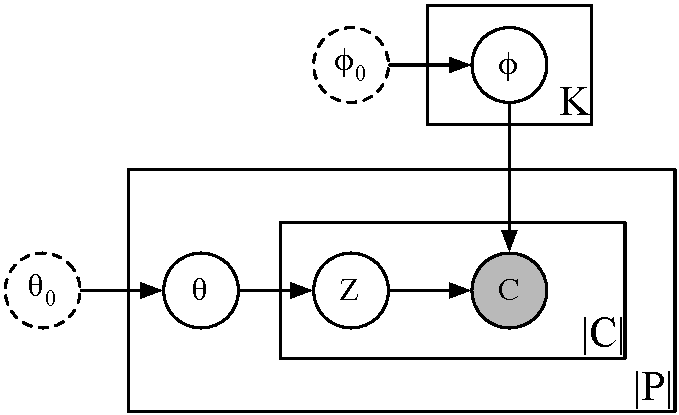
\includegraphics[scale=0.75]{pyp_clustering/np_plate.pdf}
\vspace{-0.3cm}
\end{center}
\caption{Plate diagram for the nonparametric clustering model (hyperparameters omitted).  Dashed circles indicate variables that may not be present in every model.}
\label{fig:np_plate}
\end{figure}

\paragraph{Hyperparameter priors.} The hyperparameters of the PYPs in our models are treated as random variables whose values are inferred from the data and the priors used to characterize the values we expect them to take on.  Since we have only a poor prior understanding about what their appropriate values should be, we use vague priors: discount parameters, $a_{(\cdot)}$, are drawn from a uniform Beta distribution ($a_{(\cdot)} \sim \textrm{Beta}(1,1)$) and concentration parameters, $b_{(\cdot)}$, are drawn from a Gamma distribution ($b_{(\cdot)} \sim \textrm{Gamma}(1,1)$).

\subsection{Inference}

Inference in the nonparametric clustering models was performed using Gibbs sampling \citep{geman:1984}, with the continuous parameters ($\theta_{\p}$, $\phi_z$, etc.) integrated out \citep{blunsom:2009}.  For the experiments reported below, we sampled for 1,000 iterations.  The initial state of the sampler was created by assigning every context in a phrase entirely to a random category.

Values for the PYP hyperparameters were resampled after every 10 samples of the Gibbs sampler using the range doubling slice sampling technique \citep{neal:2000,johnson:2009}.

The final sample drawn from the model was used to estimate $p(z|\textbf{c},\p)$, and each phrase occurrence was labelled with the $z$ that maximized this probability.

\section{Experiments}

This section reports a number of experiments carried out to test the quality of the grammars learned using our nonparametric cluster models.

\subsection{Corpora}

The experiments reported in this section were carried out primarily on a small Chinese-English corpus from the travel and tourism domain \citep{btec} and a more general-domain Urdu-English corpus, made available by the US National Institute of Standards and Technology (NIST) for the Open MT Evaluation.\footnote{http://www.itl.nist.gov/iad/mig/tests/mt/} Table~\ref{tab:corpbtecur} provides statistics about the training and test data used in the experiments reported in this section. Translation quality evaluation is reported using case-insensitive \textsc{bleu} \citep{bleu} with the number of references given in Table~\ref{tab:corpbtecur}.

\begin{table}[h]
\caption{Training corpus statistics for BTEC Chinese-English and the NIST Urdu-English data sets.}
\begin{center}
\begin{tabular}{l|r|r}
& BTEC & Urdu \\
\hline
Sentences & 44,016 & 51,214 \\
English types & 9,555 & 31,492 \\
English tokens & 364,297 & 968,013 \\
Foreign types & 13,664 & 33,757 \\
Foreign tokens & 333,438 & 1,052,260 \\
\hline
Development sentences & 1,006 & 882 \\
Test sentences & 506 & 883 \\
Num. references & 16 & 4
\end{tabular}
\end{center}
\label{tab:corpbtecur}
\end{table}%

\subsection{Baseline and benchmark systems}

We provide two baseline systems: a single-category system constructed using the procedure described by \cite{chiang:2007} and a system constructed by assigning categories to each phrasal occurrence in the training data.  Additionally, we provide a benchmark system using supervised English (target) language parse trees \citep{samt}.  Table~\ref{tab:npbaselines} summarizes these baseline conditions.

\begin{table}[h]
\caption{Baseline systems}
\begin{center}
\begin{tabular}{r|c|c}
& BTEC & Urdu \\
\hline
Single category \citep{chiang:2007} & 57.0 & 21.1 \\
\hline
Random ($K=10$) & 56.0 & \\
Random ($K=25$) & 55.4 & 19.7 \\
Random ($K=50$) &  55.3 & \\
\hline
Supervised \citep{samt} & 57.8 & 24.5
\end{tabular}
\end{center}
\label{tab:npbaselines}
\end{table}%


\subsection{Number of categories}

\subsection{Context types}


